\chapter{Python Packages}
Python has a rich ecosystem of libraries for scientific computing, data analysis, and geospatial processing. This chapter introduces important packages that complement Python’s core functionality, providing efficient tools for working with structured data, performing computations, and visualizing results.


\section{Review of the Python Standard Library}
Python includes a comprehensive standard library that provides built-in functionality for various tasks. The following table lists some of the most commonly used standard library modules:

\begin{center}
\begin{tabular}{|l|p{10cm}|}
\hline
\textbf{Module} & \textbf{Description} \\
\hline
os & Provides functions for interacting with the operating system. \\
sys & Gives access to system-specific parameters and functions. \\
math & Offers mathematical functions such as trigonometry, logarithms, and factorial. \\
random & Generates pseudo-random numbers and selections. \\
datetime & Handles date and time manipulation. \\
collections & Provides specialized container datatypes like namedtuples and defaultdicts. \\
itertools & Implements fast, memory-efficient iterators. \\
functools & Contains higher-order functions like memoization (lru\_cache). \\
json & Allows parsing and generation of JSON data. \\
tempfile & Creates temporary files and directories. \\
logging & Offers flexible logging utilities. \\
argparse & Parses command-line arguments. \\
shutil & Performs high-level file operations. \\
pathlib & Modern alternative to os.path for handling filesystem paths. \\
subprocess & Runs shell commands and external processes. \\
thre@ding & Provides concurrency using threads. \\
multiprocessing & Supports parallel execution of code. \\
asyncio & Provides asynchronous I/O and event loops. \\
http & Supports HTTP client and server operations. \\
urllib & Fetches data across the web. \\
sqlite3 & Provides a lightweight database engine. \\
re & Implements regular expressions. \\
\hline
\end{tabular}
\end{center}

\subsection{Working with the OS and Filesystem}
The \texttt{os} and \texttt{pathlib} modules allow interaction with the operating system and filesystem.

\begin{codeonly}{Listing Files in a Directory}
import os

# List all files in the current directory
files = os.listdir('.')
print(files)
\end{codeonly}

\begin{codeonly}{Using Pathlib for File Paths}
from pathlib import Path

# Create a path object and check if a file exists
path = Path("example.txt")
print("File exists:", path.exists())
\end{codeonly}

\subsection{Working with JSON Data}
The \texttt{json} module is used to parse and generate JSON data.

\begin{codeonly}{Parsing and Writing JSON Data}
import json

data = {"name": "Alice", "age": 30}
json_str = json.dumps(data)
print(json_str)

# Convert JSON string back to dictionary
decoded = json.loads(json_str)
print(decoded["name"])
\end{codeonly}

\subsection{Running External Commands}
The \texttt{subprocess} module allows running system commands from Python.

\begin{codeonly}{Executing a Shell Command}
import subprocess

# Run a shell command and capture its output
result = subprocess.run(["echo", "Hello, World!"], capture_output=True, text=True)
print(result.stdout)
\end{codeonly}

\subsection{Using Regular Expressions}
The \texttt{re} module provides powerful pattern matching capabilities.

\begin{codeonly}{Matching Patterns with Regular Expressions}
import re

text = "My email is example@example.com"
match = re.search(r"[\w.-]+@[\w.-]+", text)
if match:
    print("Found email:", match.group())
\end{codeonly}

This section has introduced key components of the Python standard library, demonstrating their practical usage through examples.


%==============================================================================
%
%==============================================================================
\section{Xarray - Multi-dimensional labled Data}
Xarray is a powerful library designed for working with multi-dimensional labeled data. It is particularly useful for handling NetCDF files and scientific datasets, making it an essential tool for climate and weather data analysis.

\subsection{Creating and Manipulating Xarray DataArrays}
An Xarray DataArray is a fundamental data structure representing labeled, multi-dimensional arrays.

\begin{codeonly}{Creating a DataArray}
import xarray as xr
import numpy as np

# Create a simple DataArray
data = np.random.rand(4, 3)
da = xr.DataArray(data, dims=("time", "location"), coords={"time": range(4), "location": ['A', 'B', 'C']})
print(da)
\end{codeonly}

\subsection{Using Xarray for NetCDF Files}
Xarray provides seamless integration with NetCDF files for reading and writing datasets.

\begin{codeonly}{Reading a NetCDF File}
dataset = xr.open_dataset("example.nc")
print(dataset)
\end{codeonly}

\begin{codeonly}{Writing a NetCDF File}
dataset.to_netcdf("output.nc")
\end{codeonly}

\subsection{Data Selection and Operations}
Xarray allows intuitive selection and computation on data.

\begin{codeonly}{Selecting Data by Coordinates}
selected = da.sel(time=2)
print(selected)
\end{codeonly}

\begin{codeonly}{Applying Mathematical Operations}
mean_value = da.mean(dim="time")
print(mean_value)
\end{codeonly}

\section{Pandas - Data Frames and Analysis Package}
Pandas is a fundamental package for data analysis, offering powerful tools for manipulating tabular data similar to spreadsheets or SQL databases.

\subsection{Creating DataFrames}

\begin{codeonly}{Creating a Pandas DataFrame}
import pandas as pd

data = {"A": [1, 2, 3], "B": [4, 5, 6]}
df = pd.DataFrame(data)
print(df)
\end{codeonly}

\subsection{Data Selection and Filtering}

\begin{codeonly}{Filtering Data}
filtered = df[df["A"] > 1]
print(filtered)
\end{codeonly}

\section{SciPy Scientific Computing, Optimization and Statistics}
SciPy extends NumPy with additional functionality for scientific computing, such as optimization, signal processing, and statistical analysis.

\subsection{Optimization Example}

\begin{codeonly}{Finding a Minimum Using SciPy}
from scipy.optimize import minimize

def func(x):
    return (x - 3) ** 2

result = minimize(func, x0=0)
print(result.x)
\end{codeonly}

\section{Scikit-Learn - Machine Learning, Classifiation, Regression}
Scikit-learn is a machine learning library that provides tools for classification, regression, clustering, and preprocessing.

\subsection{Fitting a Linear Model and Clustering Algorithms}

\begin{codeonly}{Linear Regression with Scikit-Learn}
from sklearn.linear_model import LinearRegression
import numpy as np

X = np.array([[1], [2], [3], [4]])
y = np.array([2, 3, 5, 7])

model = LinearRegression()
model.fit(X, y)
print("Predictions:", model.predict(X))
\end{codeonly}

The notebook \texttt{scikit-learn\_cth\_clustering.ipynb} provides a compact demonstration of hierarchical clustering on synthetic cloud top height (CTH) data. It uses agglomerative clustering to group similar CTH profiles and evaluates the results visually.

\begin{enumerate}[label=\textbf{Step \arabic*:}, leftmargin=2cm]

\item \textbf{Dataset Preparation:} The notebook loads or generates sample data representing CTH structures. These are likely extracted from satellite or model fields, reshaped into 1D or 2D patterns suitable for clustering.

\item \textbf{Hierarchical Clustering:} Using \texttt{AgglomerativeClustering} from \texttt{scikit-learn}, the notebook clusters the CTH patterns into a small number of representative types. This helps identify structural differences in convective growth.

\begin{center}
    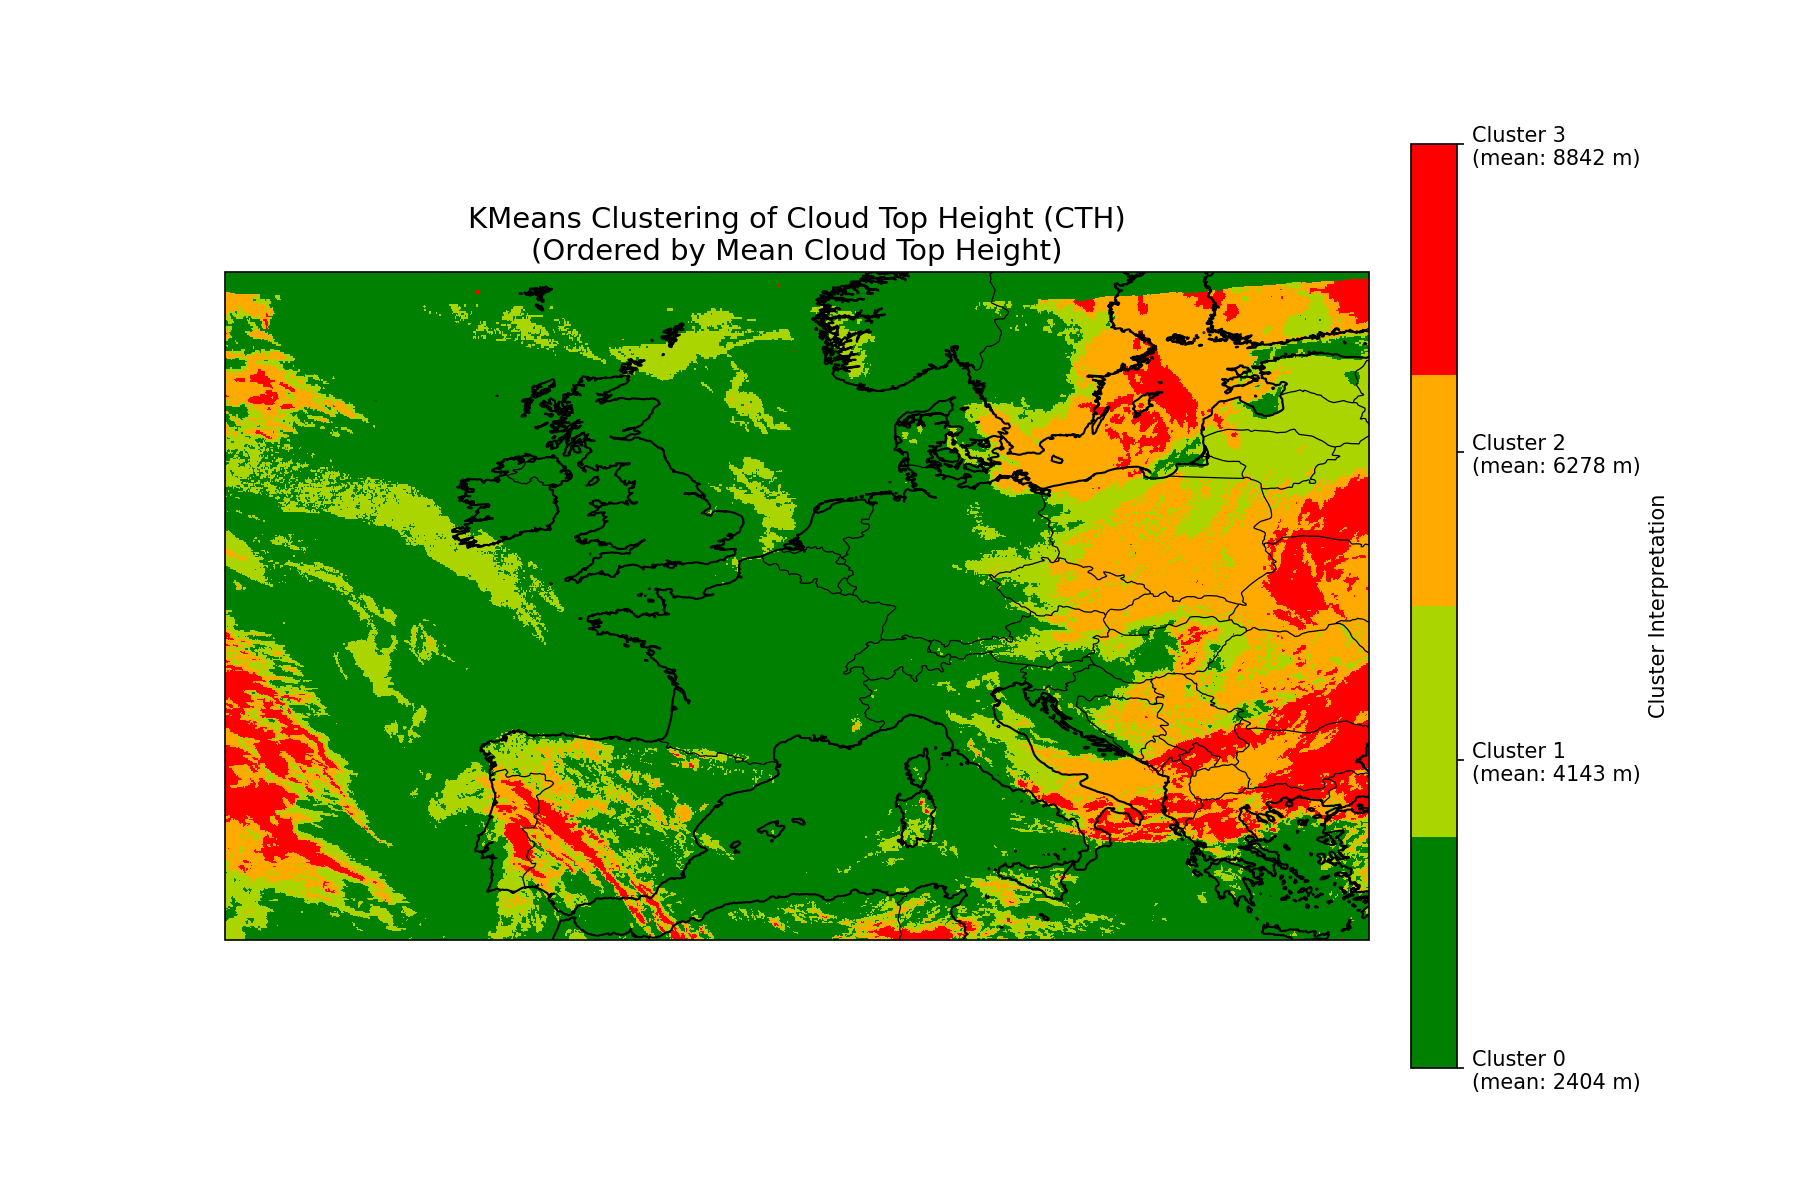
\includegraphics[width=0.7\textwidth]{images/cth_clusters_ordered.png}
    \captionof{figure}{Clustered convective profiles, sorted and labeled.}
\end{center}

\item \textbf{Comparison of Results:} To validate the clustering, side-by-side comparisons are made showing original vs. clustered versions, or showing cluster representatives.

\begin{center}
    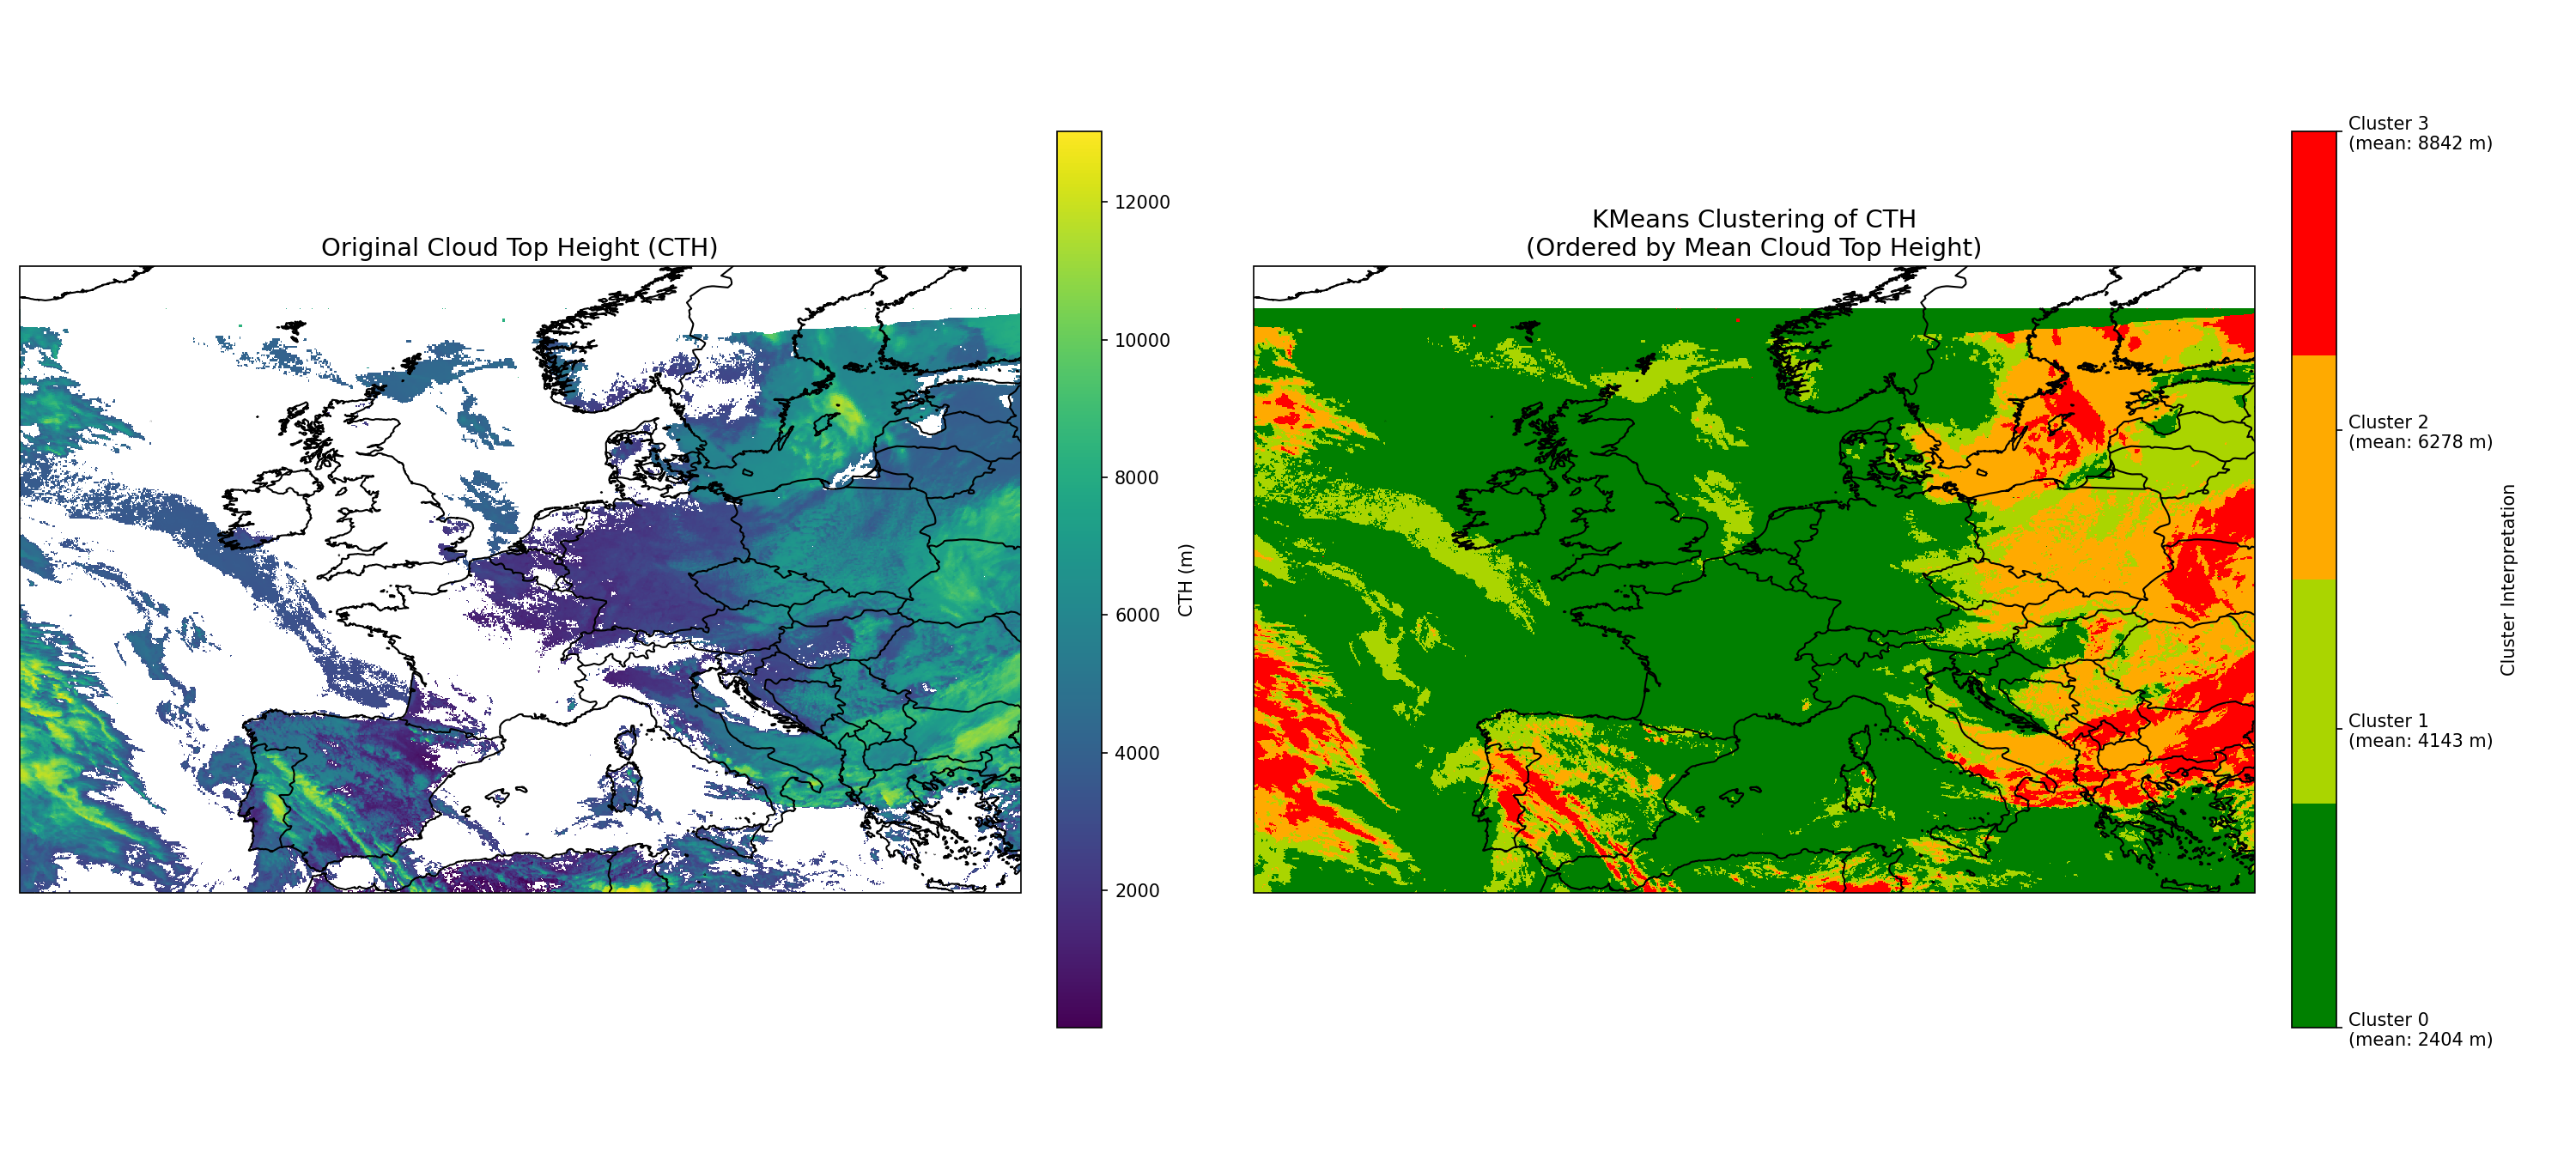
\includegraphics[width=0.7\textwidth]{images/cth_comparison_side_by_side.png}
    \captionof{figure}{Side-by-side comparison of original and clustered convective patterns.}
\end{center}

\item \textbf{Visual Interpretation:} The notebook further evaluates clusters by plotting their motion and structure. For example, flow vectors and growth regions may be overlaid.

\begin{center}
    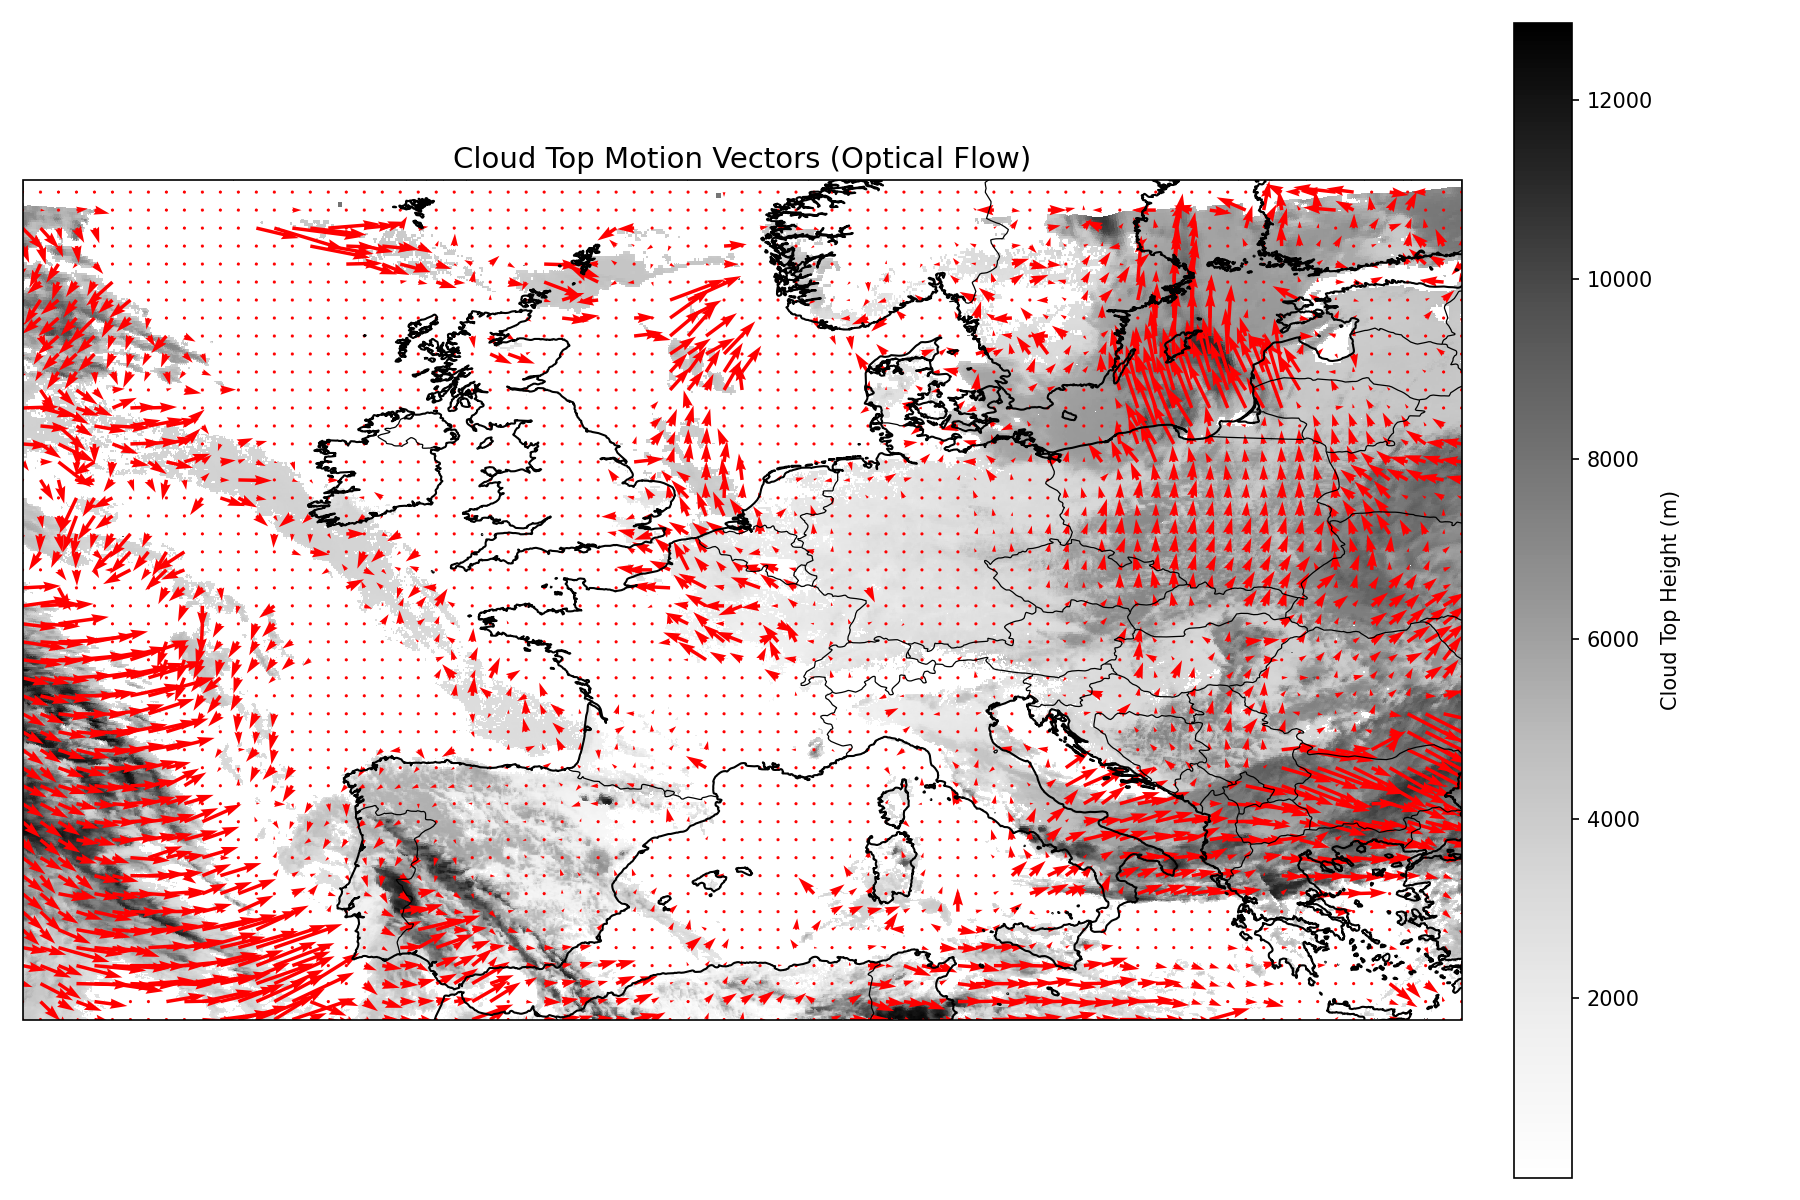
\includegraphics[width=0.7\textwidth]{images/cth_motion_vectors.png}
    \captionof{figure}{Estimated motion vectors over convective regions.}
\end{center}

\begin{center}
    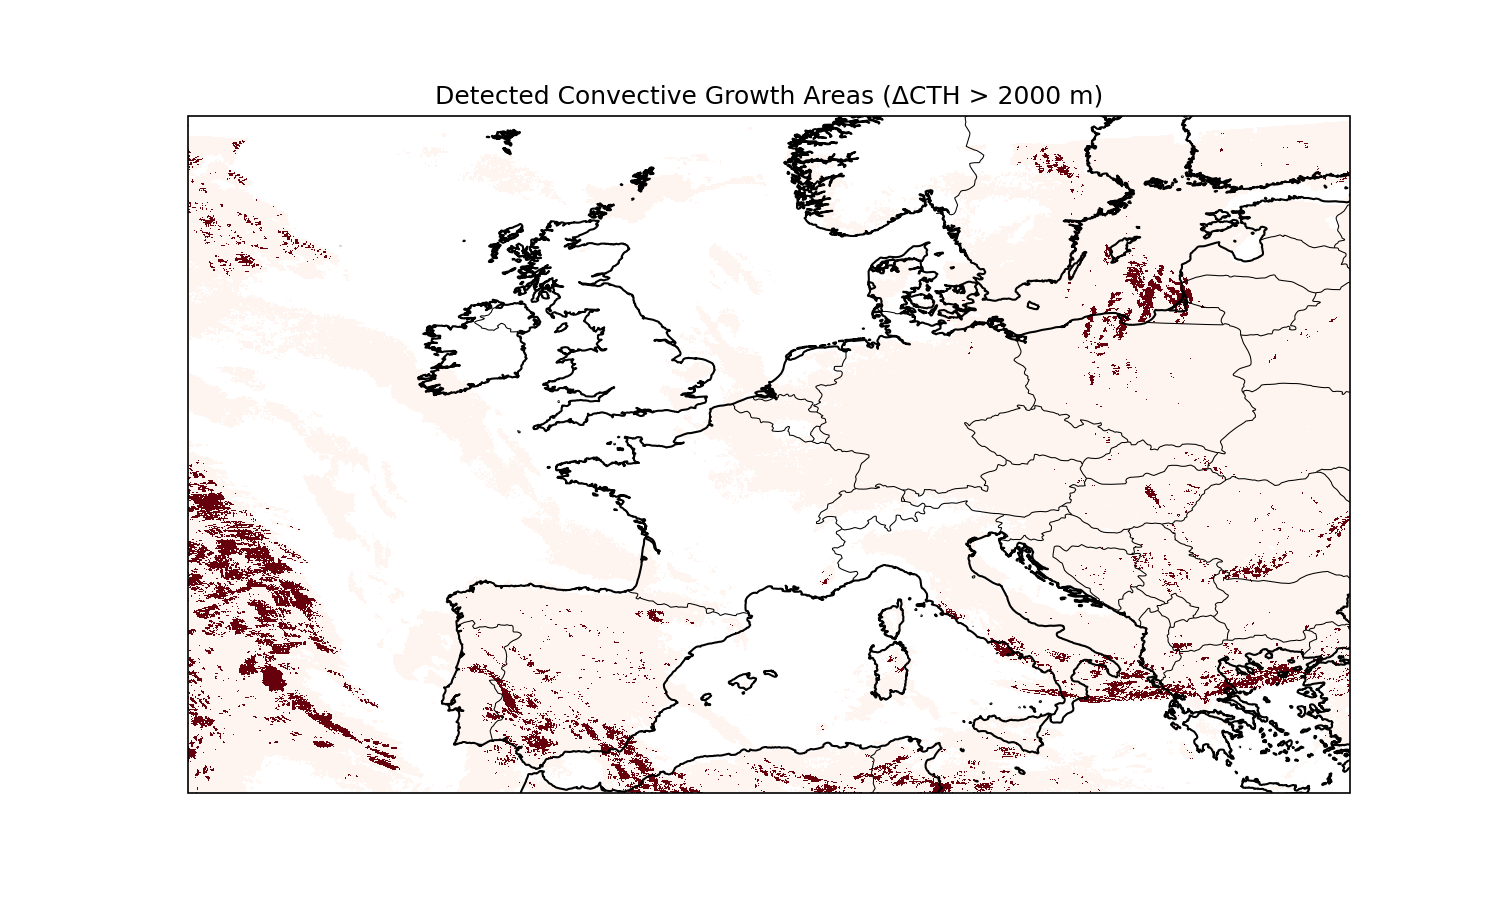
\includegraphics[width=0.7\textwidth]{images/cth_convective_growth.png}
    \captionof{figure}{Identification of regions with rapid vertical growth in CTH.}
\end{center}

\item \textbf{Map-Based Output:} Final outputs show maps of maximum change, differences, and derived quantities based on the clustering.

\begin{center}
    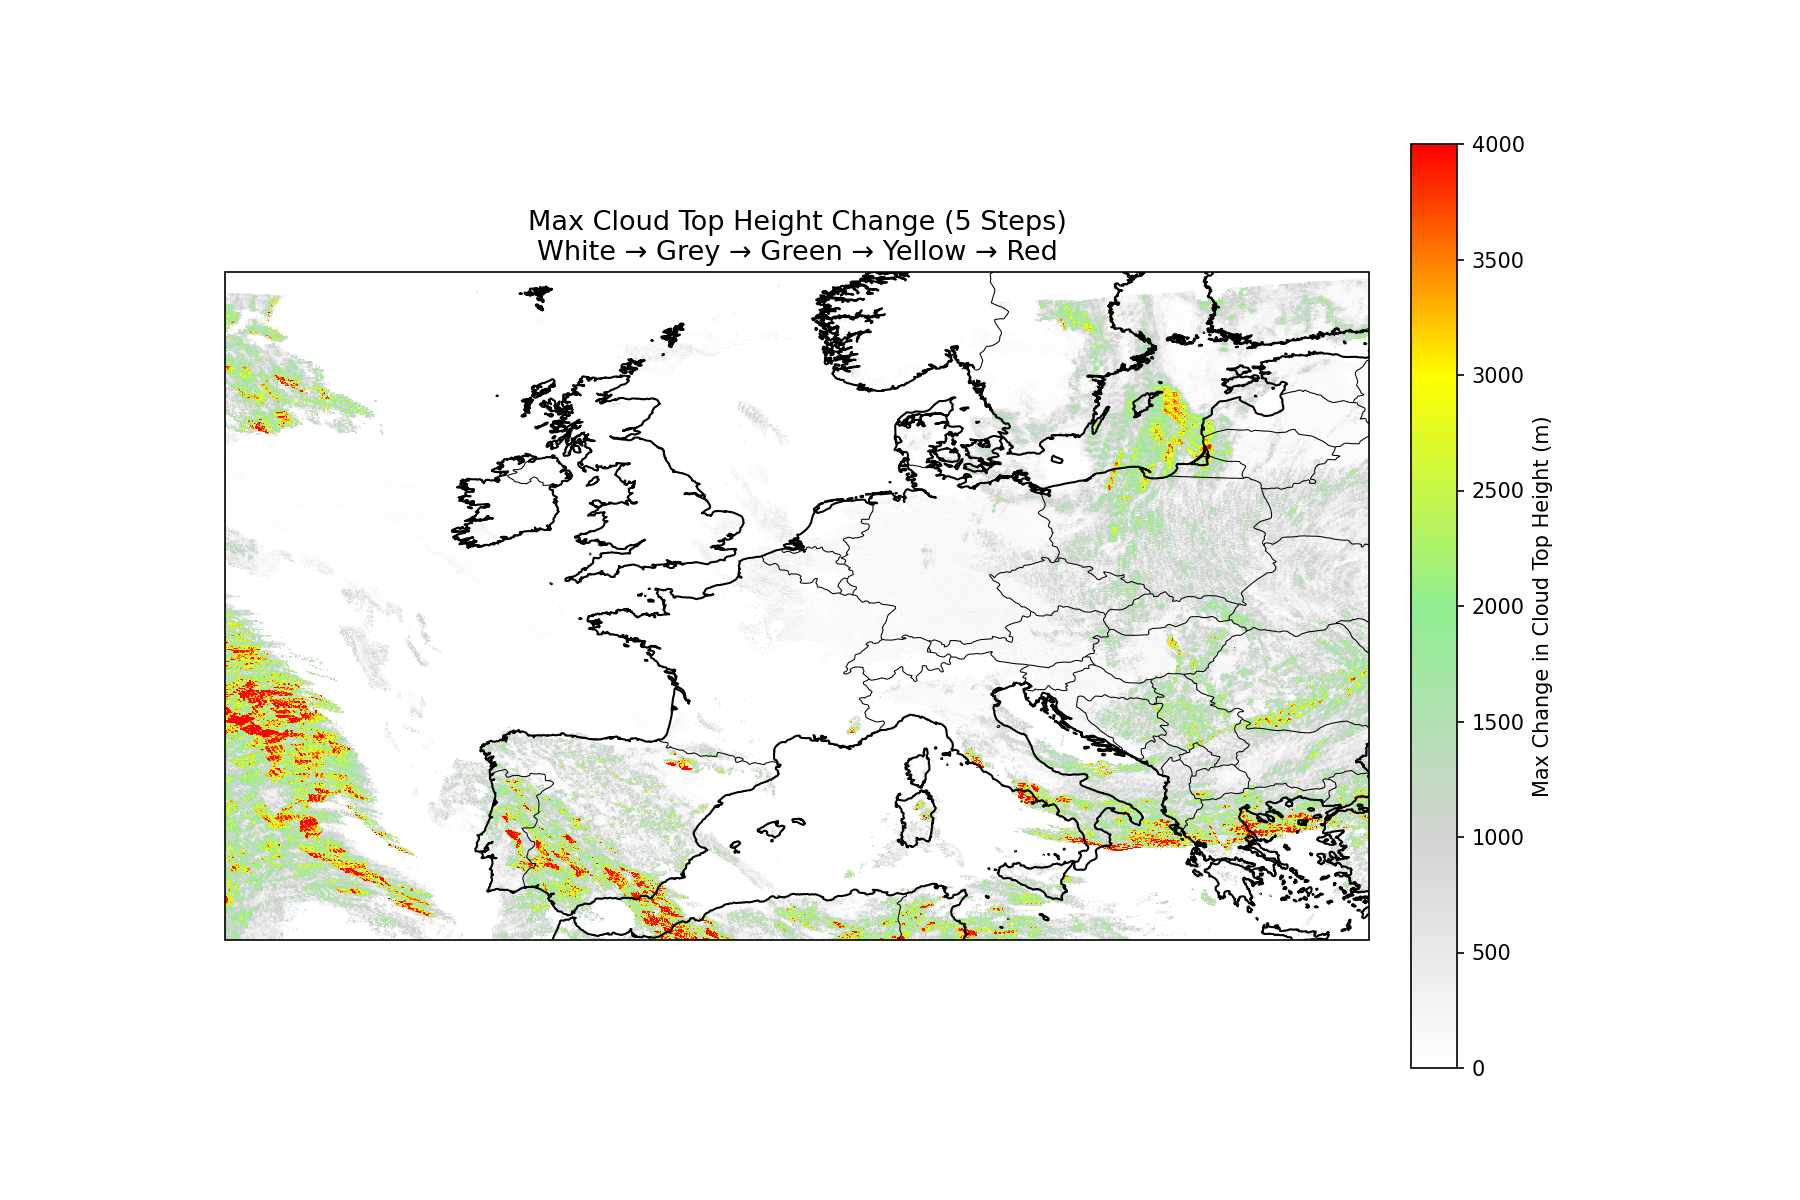
\includegraphics[width=0.7\textwidth]{images/cth_max_change_map.png}
    \captionof{figure}{Map showing maximum CTH changes across the domain.}
\end{center}

\begin{center}
    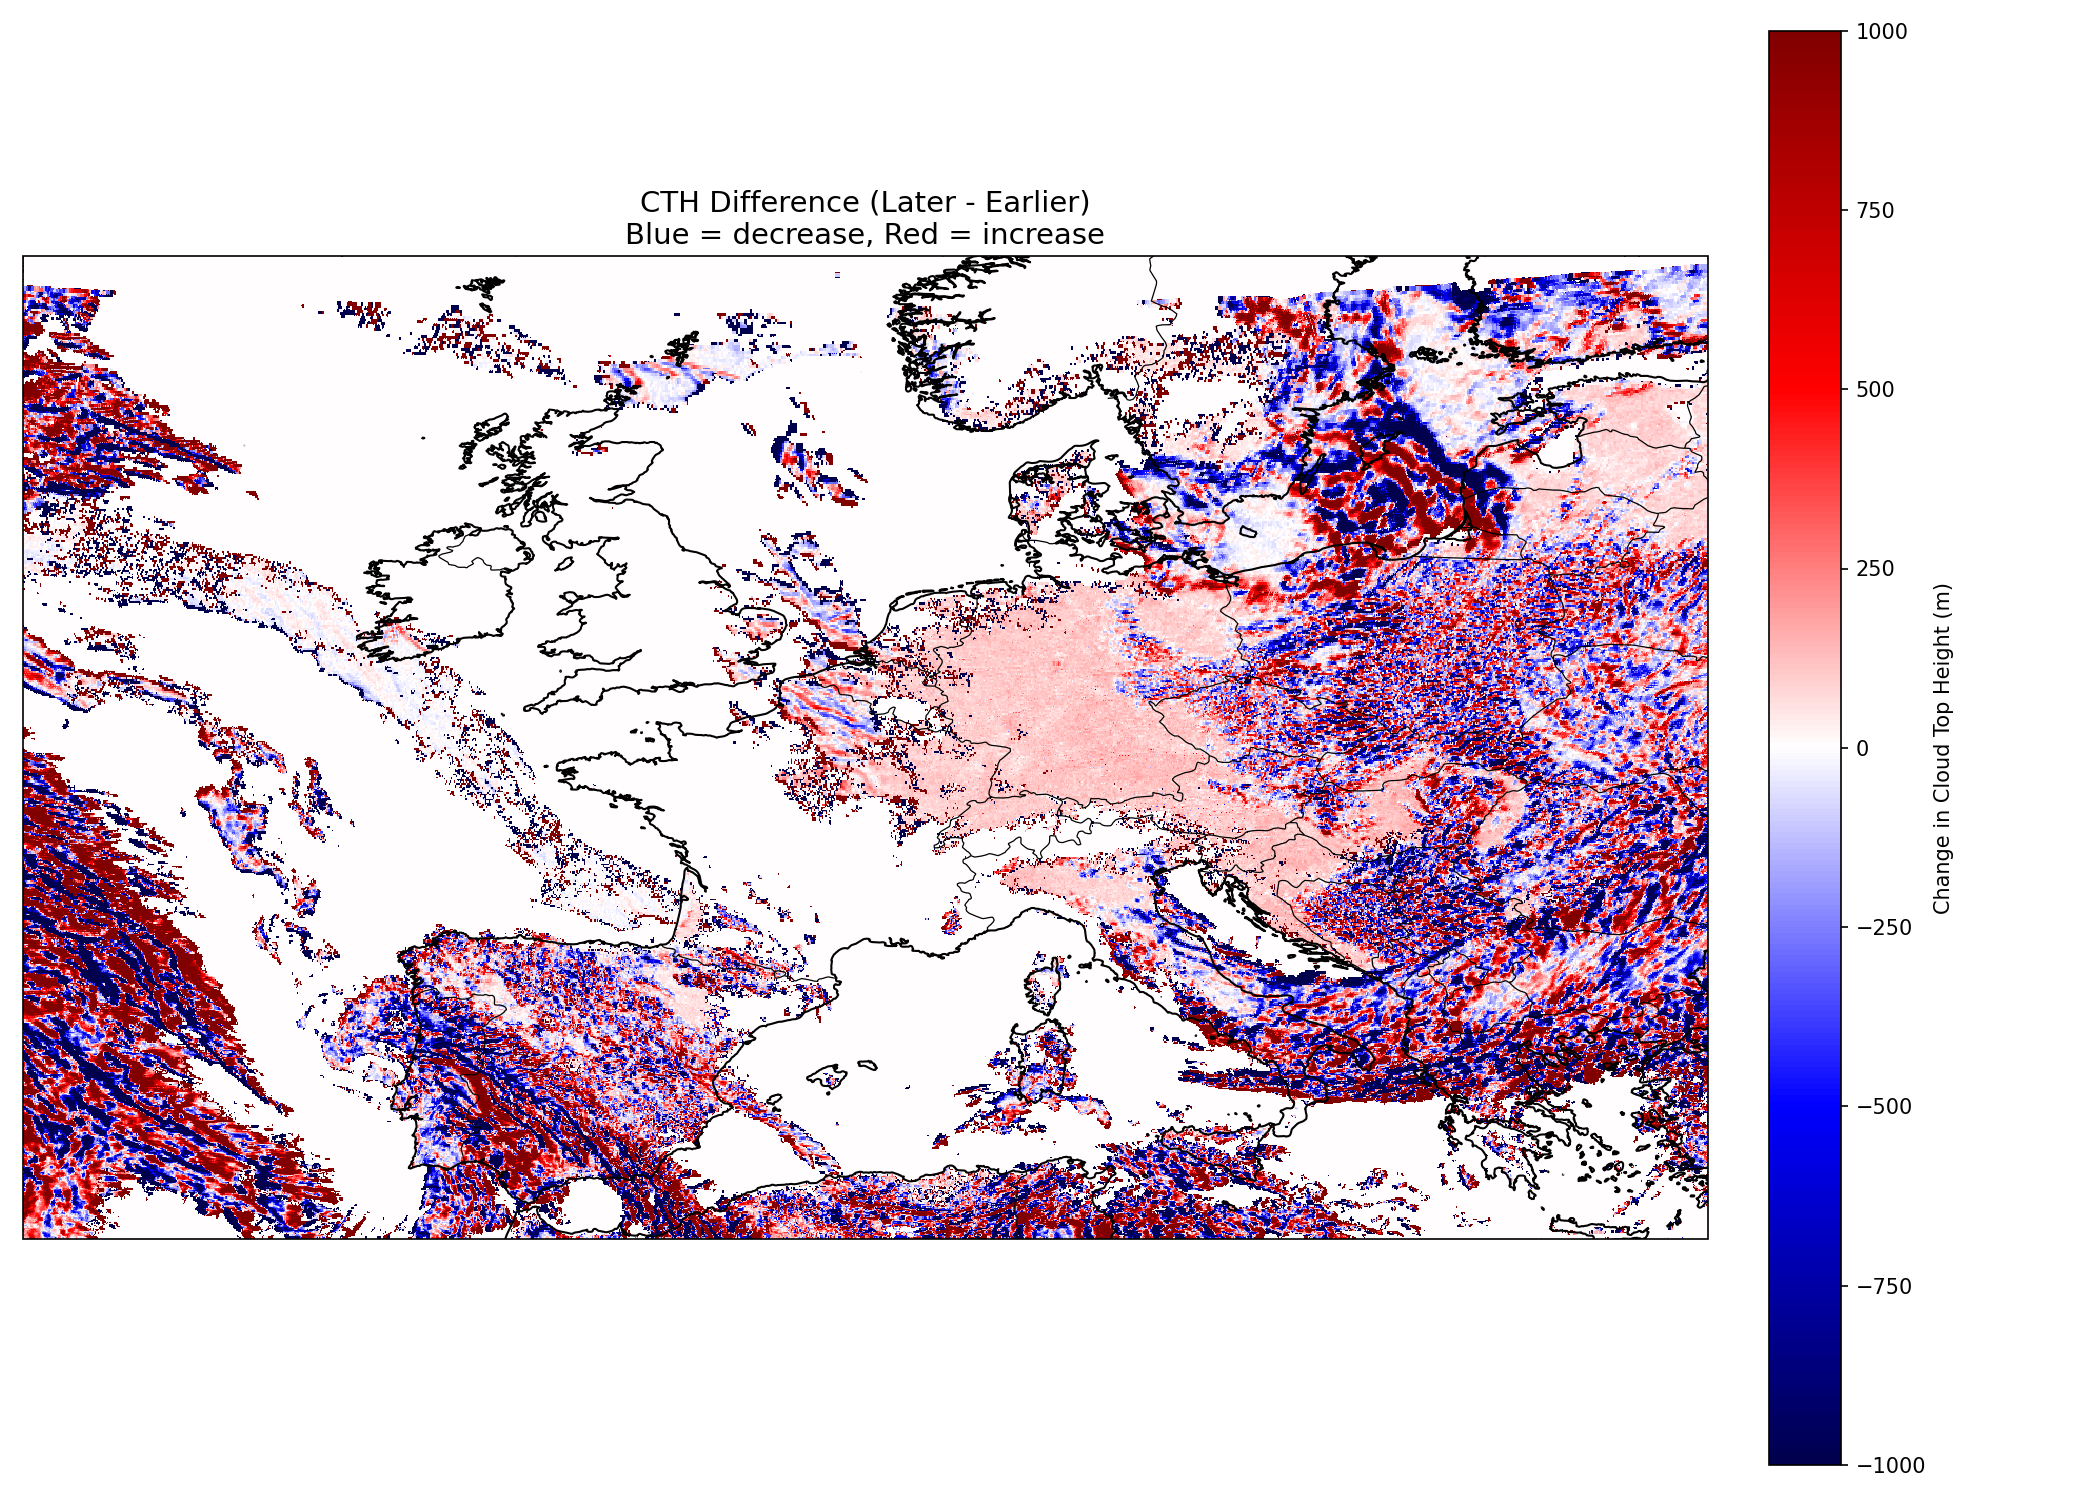
\includegraphics[width=0.7\textwidth]{images/cth_difference_map.png}
    \captionof{figure}{Difference map between cluster means and actual values.}
\end{center}

\end{enumerate}

The combination of clustering and visualization in this notebook provides insight into common convective structures, their dynamics, and how they evolve over time.


